% SPDX-License-Identifier: CC-BY-SA-4.0
% Author: Matthieu Perrin
% Part: <Nom de la partie>
% Section: <Nom de la section>
% Sub-section: <Nom de la sous-section>  % (facultatif, laisser vide si non utilisé)
% Frame: <Titre de la slide>

\begingroup

\begin{frame}{Complexité d'un problème}

  \begin{block}{Classes de complexité d'un problème}
    Soit $f$ une suite de $\mathbb{N}$ dans $\mathbb{R}^+$. 
    On définit les \structure{classes de complexité} : 
    \begin{description}[$\textsc{dspace}(f)$ :]
    \item[$\textsc{dtime}(f)$ :] les problèmes décidables en temps $\mathcal{O}(f)$ \structure{par une MTD} :
      
      \vspace{-2mm}
      $$\alert{\textsc{dtime}(f) \eqdef \{\structure{\alert{L} \in \textsc{lang} \mid \exists M, L = \mathcal{L}(M) \land \alert{T_M \in \mathcal{O}(f)}} \}}$$
    \item[$\textsc{dspace}(f)$ :] les problèmes décidables en espace $\mathcal{O}(f)$ \structure{par une MTD} :

      \vspace{-2mm}
      $$\alert{\textsc{dspace}(f) \eqdef \{\structure{\alert{L} \in \textsc{lang} \mid \exists M, L = \mathcal{L}(M) \land \alert{S_M \in \mathcal{O}(f)}} \}}$$
    \end{description}
  \end{block}

  \pause
  \vspace{-1mm}
  \begin{block}{Classes de complexité importantes}

    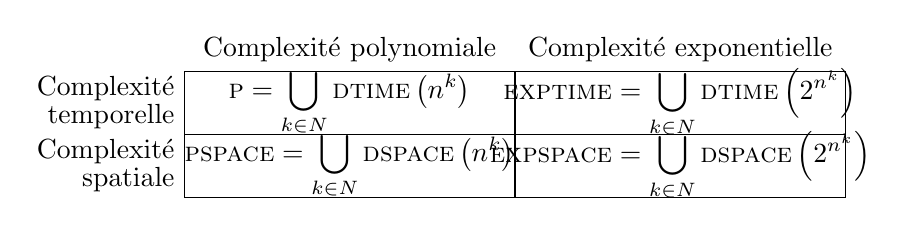
\begin{tikzpicture}[y=4mm, x=21mm]
      \draw (0,0) -- (4,0);
      \draw (0,2) -- (4,2);
      \draw (0,4) -- (4,4);
      \draw (0, 0) -- (0, 4);
      \draw (2, 0) -- (2, 4);
      \draw (4, 0) -- (4, 4);
      
      \node[align=center] at (1,3) {$\alert{\displaystyle \textsc{p} = \bigcup_{k\in \mathbb{N}} \textsc{dtime}\left(n^k\right)}$};
      \node[align=center] at (3,3) {$\alert{\displaystyle \textsc{exptime} = \bigcup_{k\in \mathbb{N}} \textsc{dtime}\left(2^{n^k}\right)}$};
      \node[align=center] at (1,1) {$\alert{\displaystyle \textsc{pspace} = \bigcup_{k\in \mathbb{N}} \textsc{dspace}\left(n^k\right)}$};
      \node[align=center] at (3,1) {$\alert{\displaystyle \textsc{expspace} = \bigcup_{k\in \mathbb{N}} \textsc{dspace}\left(2^{n^k}\right)}$};

      \node[align=center, above] at (1,4) {Complexité \structure{polynomiale}};
      \node[align=center, above] at (3,4) {Complexité \structure{exponentielle}};
      \node[align=right,  left ] at (0,1) {Complexité\\[-2pt]\structure{spatiale}};
      \node[align=right,  left ] at (0,3) {Complexité\\[-2pt]\structure{temporelle}};
    \end{tikzpicture}
    
    $$ \textsc{dtime}\left(\log(n)\right) \subsetneq \alert{\textsc{p}} \subsetneq \textsc{dtime}\left(n^{\log(n)}\right) \subsetneq \alert{\textsc{exptime}} \subsetneq \textsc{dtime}\left(n!\right) $$
  \end{block}
  
\end{frame}

\endgroup
\endinput
